\documentclass[11pt,a4paper]{article}

\usepackage[utf8]{inputenc}
\usepackage[OT4]{fontenc}
\usepackage{amsmath}
\usepackage{amssymb}
\usepackage{graphicx}
\usepackage{fullpage}

\title{Agent-based indoors virus propagation model}
\author{Jarosław Miszczak}

\begin{document}
\maketitle

%%%%%%%%%%%%%%%%%%%%%%%%%%%%%%%%%%%%%%%%%%%%%%%%%%%%%%%%%%%%%%%%%%%%%%%%%%%%%%%%
\section{Introduction}
%%%%%%%%%%%%%%%%%%%%%%%%%%%%%%%%%%%%%%%%%%%%%%%%%%%%%%%%%%%%%%%%%%%%%%%%%%%%%%%%


%%%%%%%%%%%%%%%%%%%%%%%%%%%%%%%%%%%%%%%%%%%%%%%%%%%%%%%%%%%%%%%%%%%%%%%%%%%%%%%%
\section{Agent-based model}
%%%%%%%%%%%%%%%%%%%%%%%%%%%%%%%%%%%%%%%%%%%%%%%%%%%%%%%%%%%%%%%%%%%%%%%%%%%%%%%%

\begin{figure}[ht!]
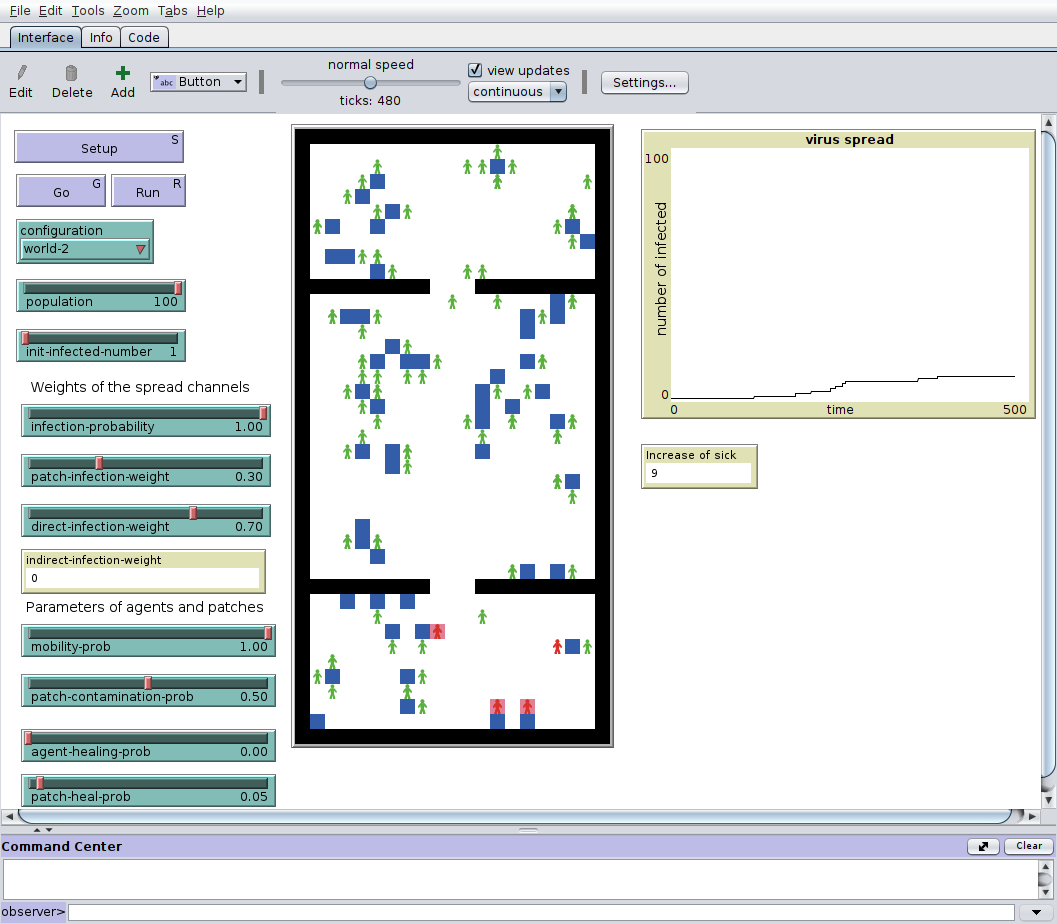
\includegraphics[width=\textwidth]{plots/model-gui.png}
\caption{User interface for the NetLogo model of indoors virus propagation with generated configuration.}
\end{figure}


%%%%%%%%%%%%%%%%%%%%%%%%%%%%%%%%%%%%%%%%%%%%%%%%%%%%%%%%%%%%%%%%%%%%%%%%%%%%%%%%
\section{Simulation results}
%%%%%%%%%%%%%%%%%%%%%%%%%%%%%%%%%%%%%%%%%%%%%%%%%%%%%%%%%%%%%%%%%%%%%%%%%%%%%%%%

\begin{figure}[ht!]
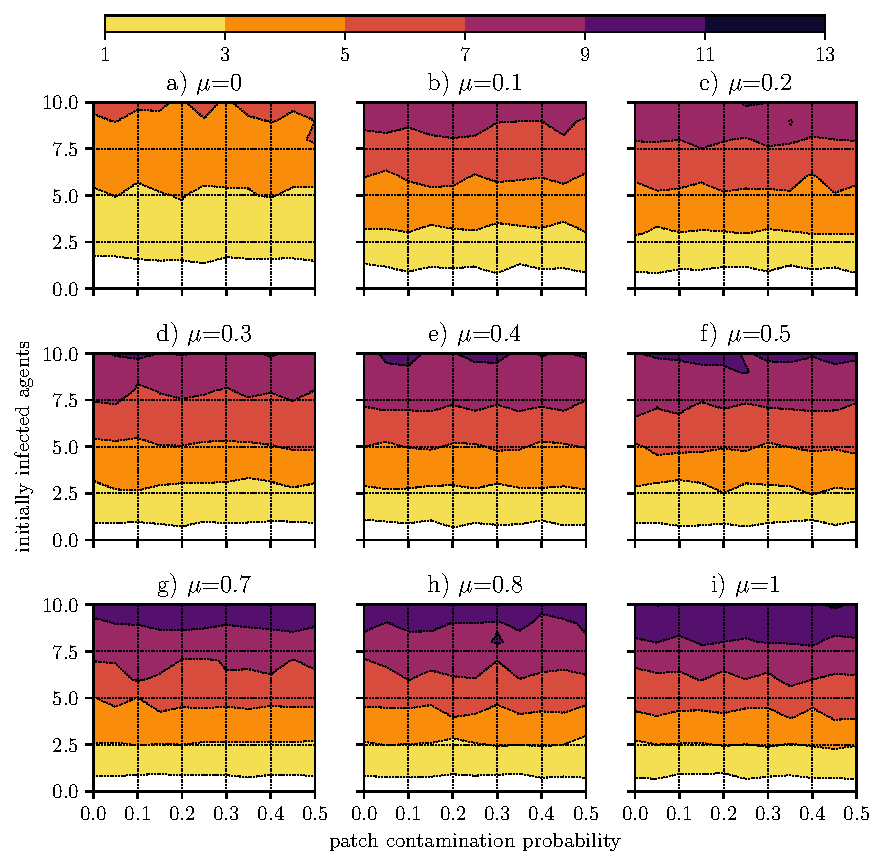
\includegraphics{plots/plot_exp6-full.pdf}
\caption{Mean increase in the number of infected agents for different values of mobility parameter $\mu$. Each plot represents the absolute increase of the number of infected agents in the population of 100 agents with different number of initially infected agents, ranging from $1$ to $10$,  and with different values of probability contaminating the items. The results were obtained by running \texttt{exp6} from \texttt{experiments-v2.xml}.}
\end{figure}

\begin{figure}[ht!]
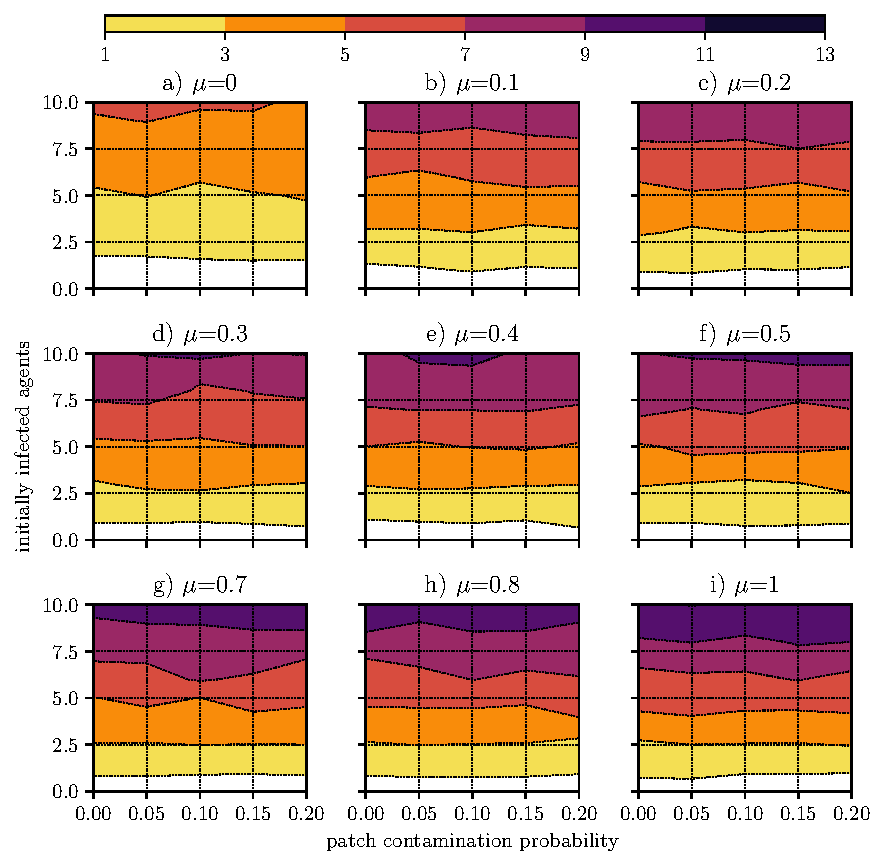
\includegraphics{plots/plot_exp6-part.pdf}
\caption{Zoomed versions of the previous plots.}
\end{figure}


\end{document}